%! Author = sbbfti
%! Date = 10/06/2020

\section{Results}\label{sec:results}

\subsection{Heat Losses, Gains, and Physiological Variables}\label{subsec:res-heat-loss-physiological}

The sensible heat loss from the skin to the environment is proportional to the difference between the \ac{t-sk} and \ac{t-op}, as shown in Equation~\ref{eq:c-r}.
Consequently, for values of \ac{t-op} higher than \ac{t-sk} the body gains sensible heat from its environment and the term \ac{c-r} becomes negative.
Figure~\ref{fig:comparison_models}A shows how sensible heat loss estimated with the \mycite{GaggeSET} and the \mycite{Jay2015} models vary as a function of \ac{t-op}, \ac{rh}, and \ac{v}.
The former model iteratively determines \ac{t-sk}, while the latter assumes it to be constant and equal to 35~$^{\circ}$C\@.
When heat gains exceed heat losses, the \mycite{GaggeSET} model estimates that some heat energy is stored in the body and consequently \ac{t-sk} increases, as shown in Figure~\ref{fig:results_model_2}A and ~\ref{fig:results_model_2}C, respectively.
This reduces the rate at which sensible heat gain increases as \ac{t-op} increases.

The values of \ac{w} for two air speeds are shown in Figure~\ref{fig:comparison_models}B\@.
The skin wettedness is allowed by the model to increase until it reaches the value of \ac{w-max}, after that, it plateaus and remains constant.
For young adults, \mycite{Jay2015} assumed \ac{w-max} to be equal to 0.65 for the `fan on' condition and 0.85 for the `fan off' condition.
From Figure~\ref{fig:comparison_models}B it can be observed that the values of \ac{w-max} estimated by the \mycite{GaggeSET} for the same air speeds are lower.
The operative temperature at which \ac{w} equals \ac{w-max} is inversely proportional to the value of \ac{rh}.

\begin{figure}[thb!]
    \centering
    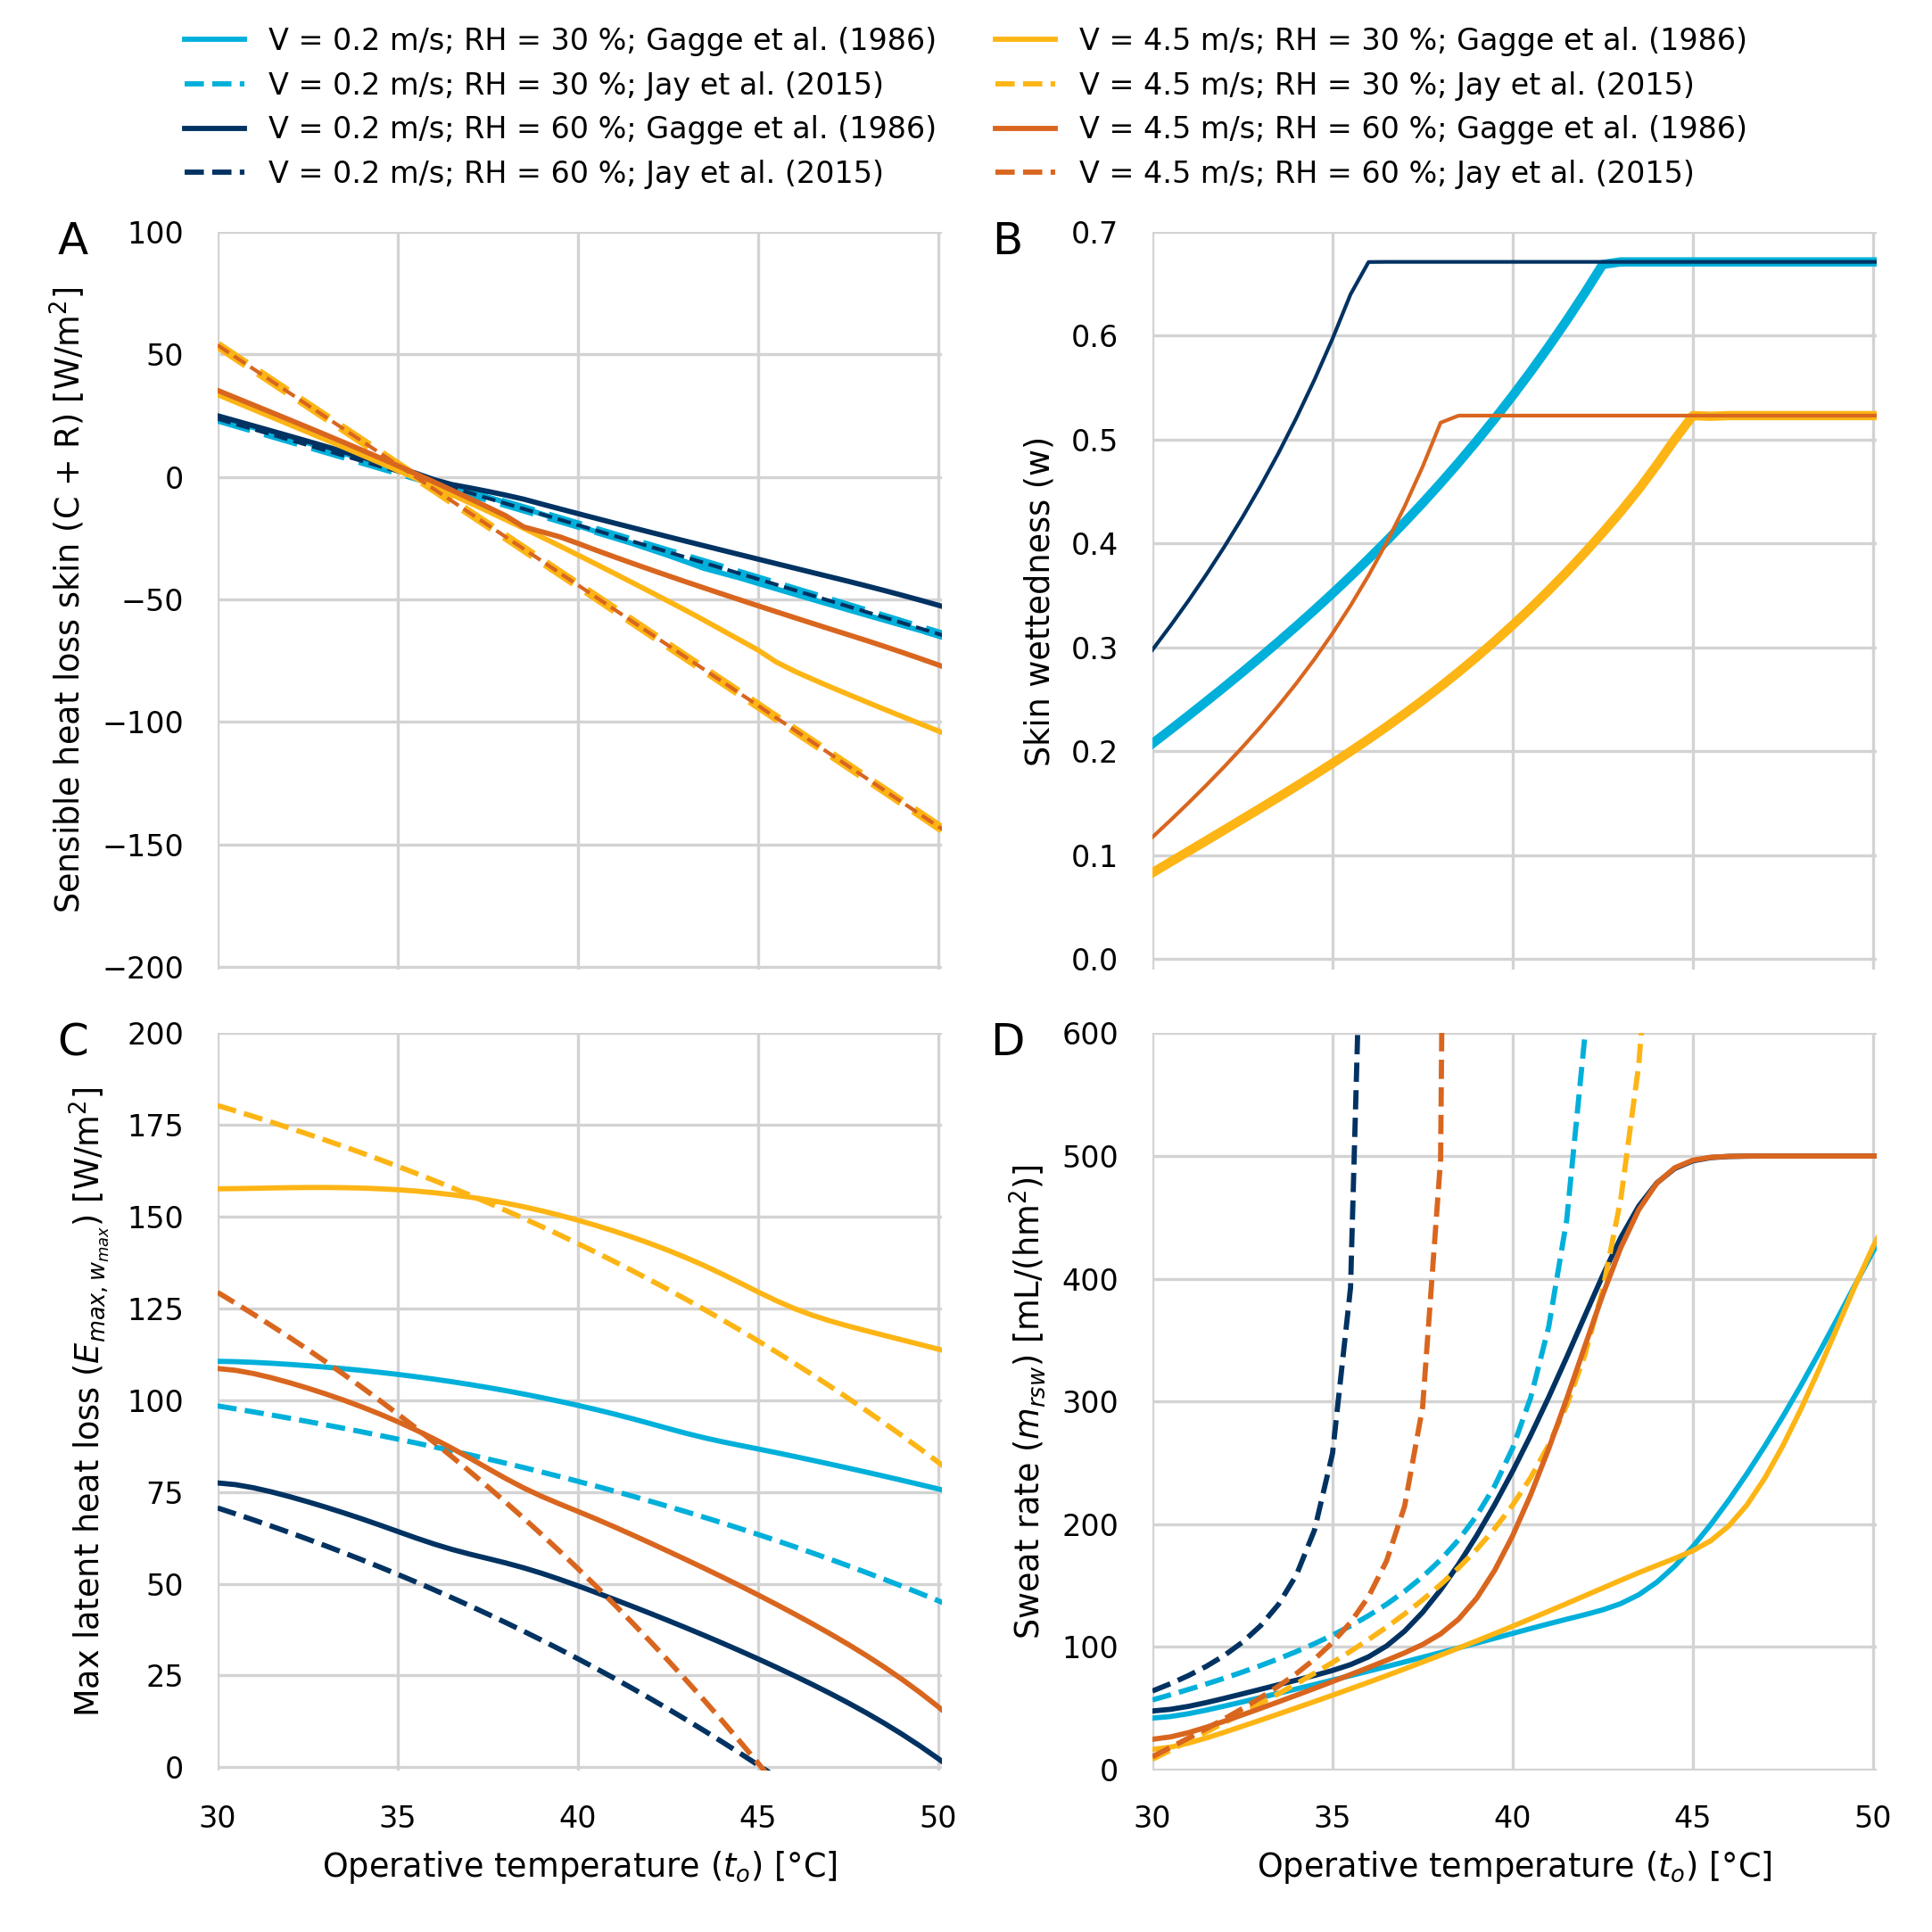
\includegraphics[width=\textwidth]{figures/comparison_models_v2}
    \caption{Results obtained with the energy models proposed by \mycite{Jay2015} and \mycite{GaggeSET}.
    Each Figure shows how a variable changes as a function of \ac{t-op} for a set combination of \ac{rh} and \ac{v}.
    Figure: A) \Acf{c-r}.
    B) \Acf{w}.
    C) \Acf{e-max} estimated using \ac{w} = \ac{w-max}.
    D) \Acf{m-sweat}.}
    \label{fig:comparison_models}
\end{figure}

% note OJ - An issue needed to be considered here is a maximum sweat rate. With high air speeds the required sweat rate to achieve the theoretical Emax might not be possible.
% the Gagge's model limits the max sweat rate at 500mL/hm2

% note Stefano - this figure it is too complex and you should select only the most important cases.

For \ac{t-op} higher than \ac{t-sk}, the negative effect that an increase in \ac{v} has on sensible heat gain is compensated by a greater increase in the \acf{e-sk} that the body can dissipate towards the surrounding environment.
For example, when \ac{t-op}~=~45~$^{\circ}$C and \ac{rh}~=~30~\%, a change in \ac{v} from 0.2 to 4.5~m/s increases (\acs{c-r}) by 29 W/m\textsuperscript{2} while increasing \ac{e-sk} by 45~W/m\textsuperscript{2}, which provides a net positive effect.

Figure~\ref{fig:comparison_models}C shows the values of \ac{e-max} estimated by replacing \ac{w} in Equation~\ref{eq:latent-skin} with \ac{w-max}.
The value of \ac{e-max} decreases as \ac{t-op} increases since \ac{p-a} grows more rapidly than \ac{p-sk}.
For a set combination of \ac{v} and \ac{t-op} the value of \ac{e-max} decreases as the value of \ac{rh} increases.
This is because humid air has a higher \ac{p-a} than dry air.
The reduction in \ac{e-max} estimated by our model is lower than the one estimated by \mycite{Jay2015} since an increase in \ac{t-sk} elevates the vapor pressure gradient between the skin and its surrounding environment.

The \acf{m-sweat} is shown in Figure~\ref{fig:comparison_models}D\@.
The difference between the results obtained with the two heat balance models can be attributed to the fact that \citeauthor{Jay2015} calculate the value of \ac{m-sweat} as a function of the required latent energy that the body should, in theory, dissipate to achieve thermal neutrality.
On the other hand, \citeauthor{GaggeSET} calculate the value of \ac{m-sweat} as a function of regulatory signals and they assume that \ac{m-sweat} cannot exceed 500~mL/h.

% note OJ It is good that a max sweat rate is included... The Jay model assumes steady-state

% note FT In the most recent paper from Jay, they assume that the max sweat rate is 440 mL/h (in their model). However, we can sweat more than 500 mL/h, for example in a field study participants exposed to 47C and 10%  sweated 691 mL/h (when fan were on) but when fan off they sweated 328g/h. Under 40C and 50% they sweated 346 and 216 g/h, with fan and no fan, respectively. Hence, only with very low humidity, high temp and fan  on people sweated more than 500. I do not know what it the max value we can sweat, I guess it would vary from person to person. Moreover, Gagge's model estimates that the a value of 500mL/h is only reached in extreme conditions (red area Figure 7) when fans should no longer be used. I am planning to add a table at the end of the

\begin{figure}[thb!]
    \centering
    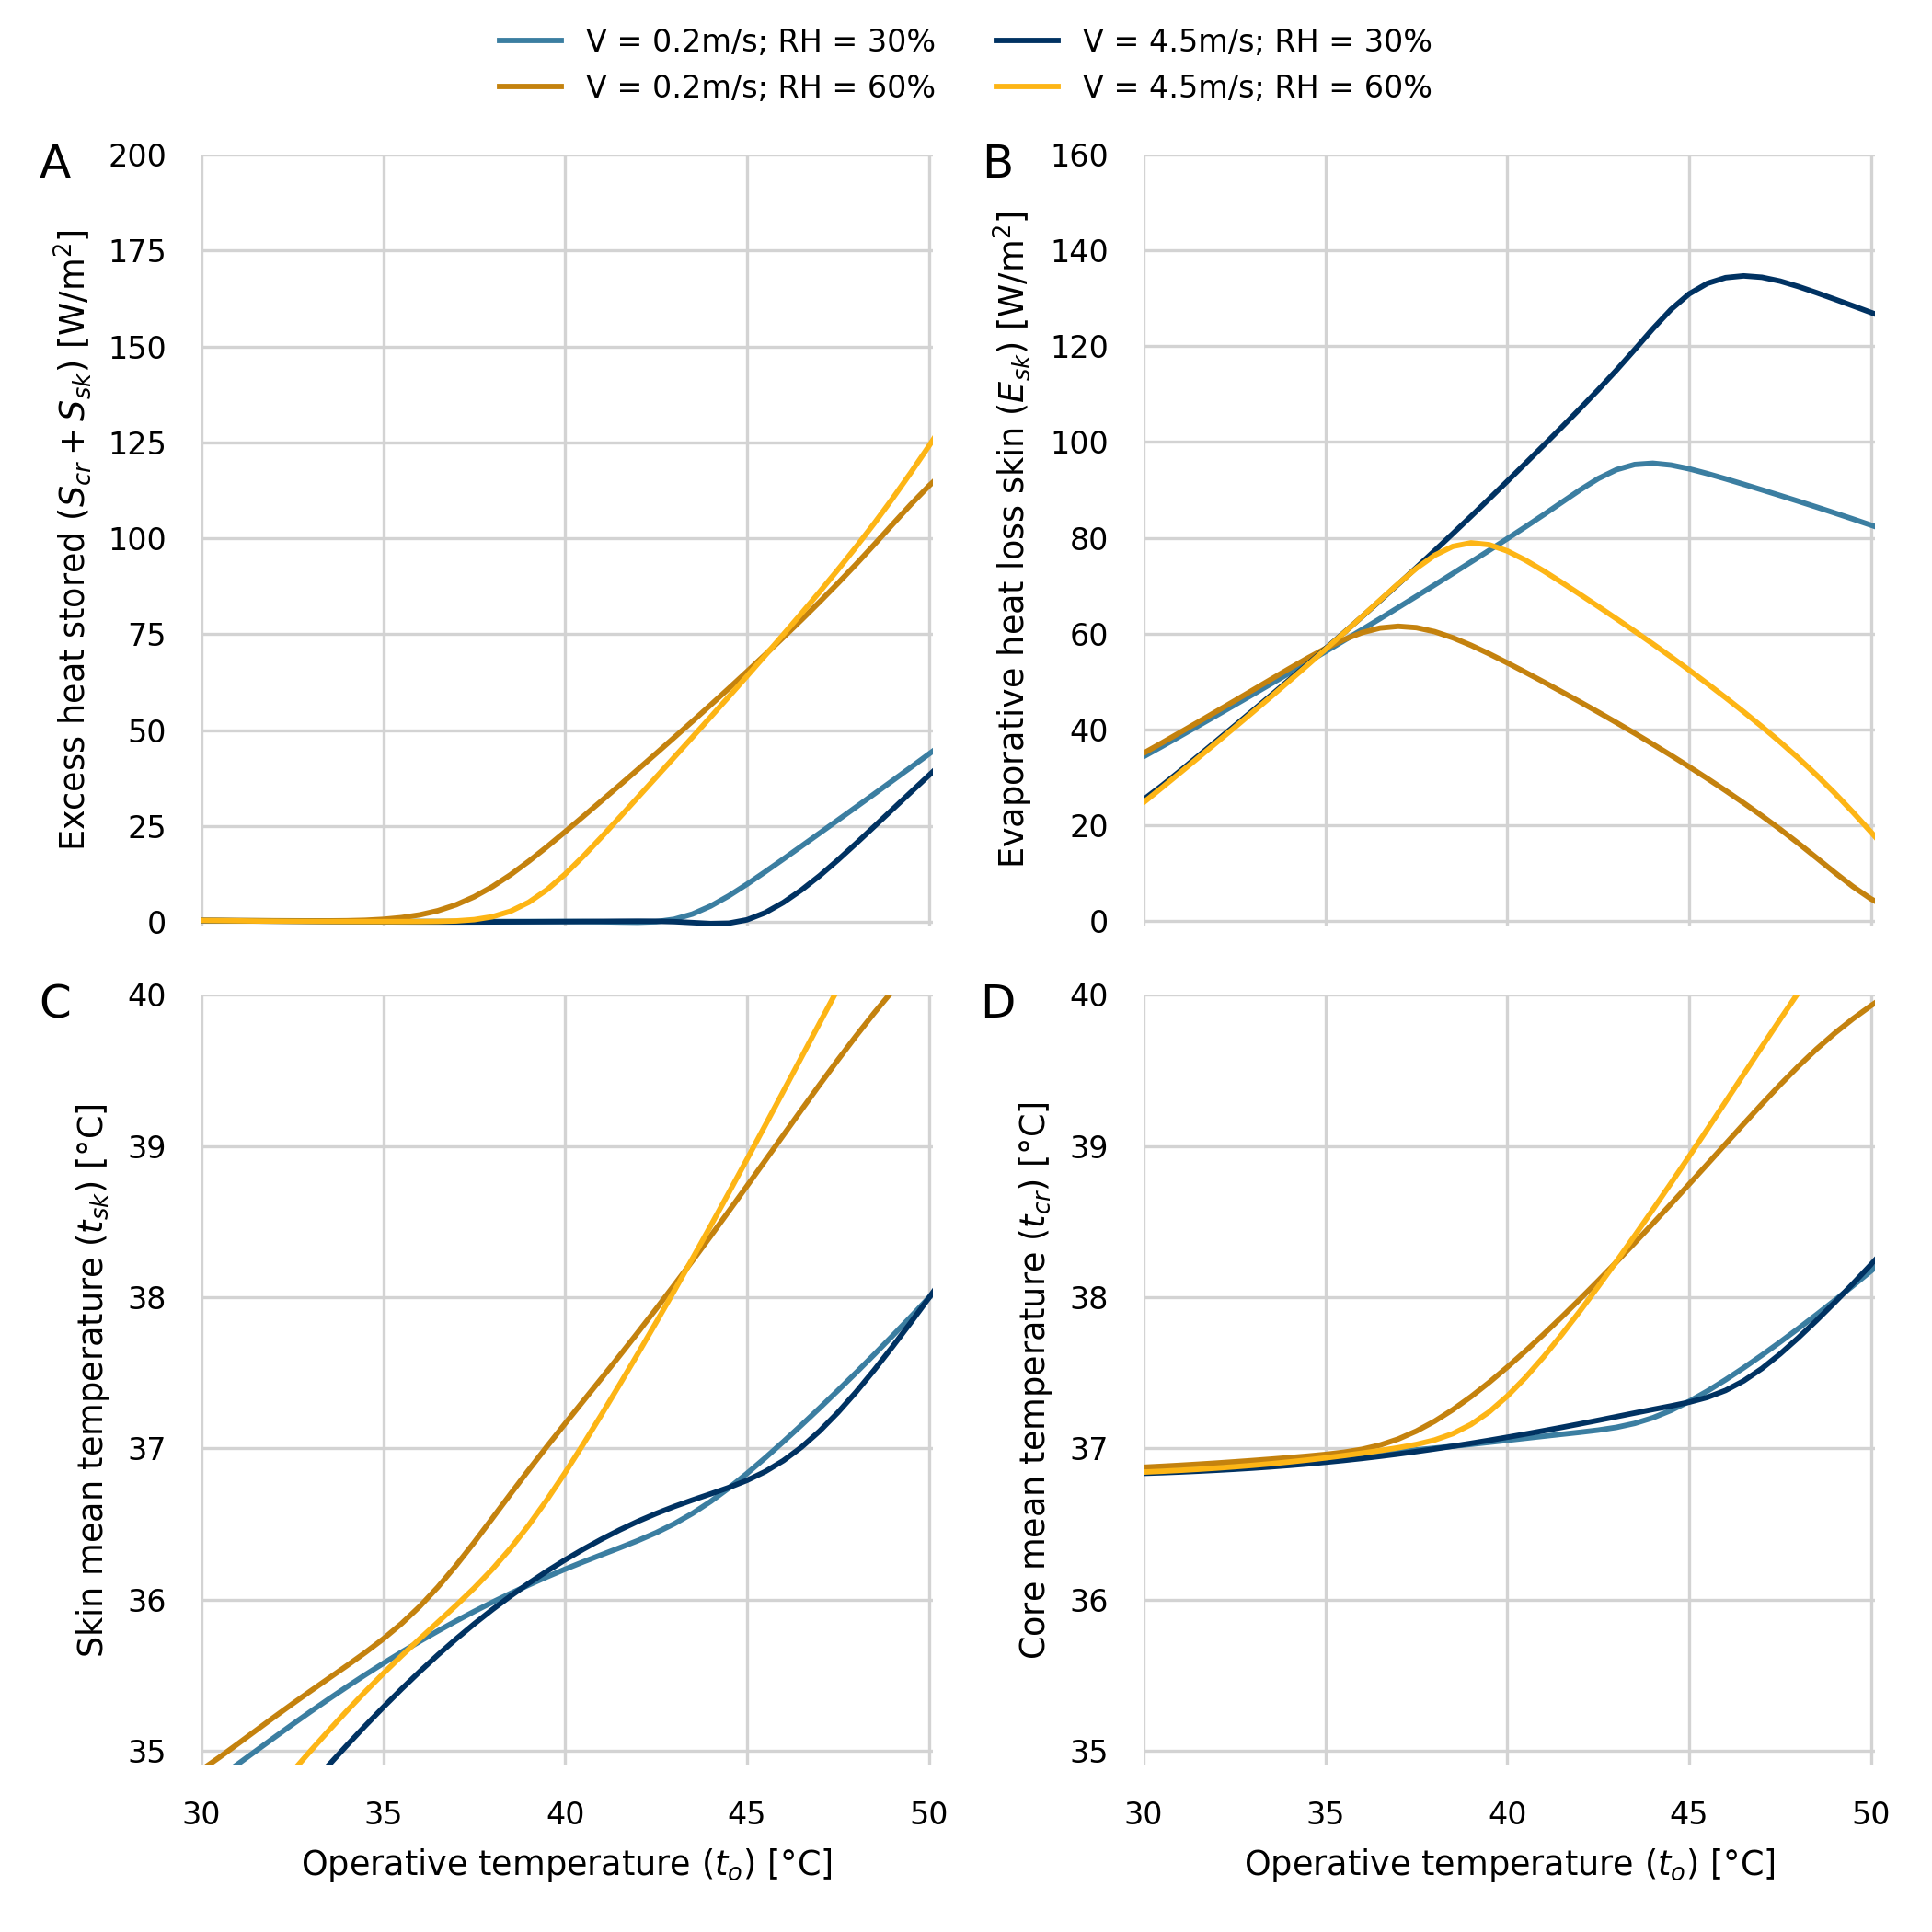
\includegraphics[width=\textwidth]{figures/results_model_2}
    \caption{Results obtained with \mycite{GaggeSET} energy model.
    Each Figure shows how a variable changes as a function of \ac{t-op} for a set combination of \ac{rh} and \ac{v}.
    Figure: A)  Excess heat stored in the human body, skin and core compartments (\ac{s-sk} + \ac{s-cr}).
    B) \Acf{e-sk}.
    C) \Acf{t-sk}.
    D) \Acf{t-cr}.}
    \label{fig:results_model_2}
\end{figure}

The excess heat stored in the human body (\acs{s-cr} + \acs{s-sk}), \ac{t-sk}, and \ac{t-cr} are shown in Figure~\ref{fig:results_model_2}A, \ref{fig:results_model_2}C, and \ref{fig:results_model_2}D, respectively.
When the body cannot longer dissipate exogenous and endogenous heat gains, the excess heat gets stored in the human body causes \ac{t-sk} and \ac{t-cr} to raise.

% note Federico to Stefano - The increase in the core temperature it is a concern, but as you can see from Figure 3 if the fans are on, the core body temperature is lower than when fans are off. This is true till a certain point when this trend is inverted and the core temperature with the fans on is higher than with the fan off. As you can see from Figure 3 the point in which the two lines intersect is the same point above which in Figure 7 we are no longer recommending to use electric fans. Hence, fans are still beneficial to use, even though people may be suffering, they are better than nothing. Moreover, from figure 3 it can be observed that the critical temperature above which core body temperature starts increasing is higher when fans are turned on, and this temperature is higher than 35C. Till that temperature the use of fans is actually good since it onsets the increase in the core temperature.

To validate the results of our model, we examined how the predicted value of \ac{t-cr} varies as a function of \ac{rh}, under a set of specific conditions as tested experimentally by \mycite{Rate2015} (e.g., \ac{t-db}~=~42~$^{\circ}$C, \ac{v}~=~4.0~m/s, \ac{clo}~=~0.35~clo, and \ac{met}~=~1.0~met).
The results are shown in Figure~\ref{fig:comparison_ravanelli}.
It should be noted that \mycite{Rate2015} only reported the core body temperature of one participant.
% note OJ We have these data though so we could share them for all participants if you think they would be helpful
% FT please share the data with us
Consequently, despite the agreement with their experimental data (mean absolute error~=~0.04~$^{\circ}$C), more quantitative data will be needed for validation.

\begin{figure}[thb!]
    \centering
    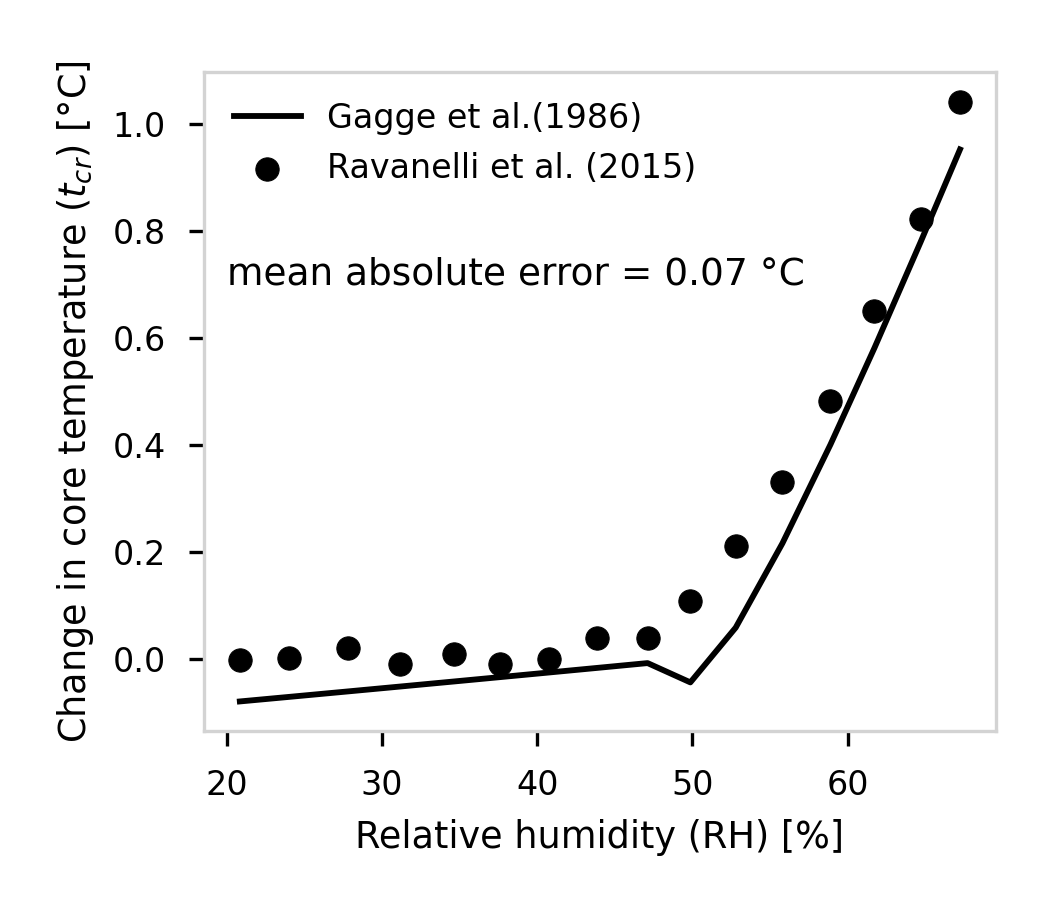
\includegraphics[width=0.5\textwidth]{figures/comparison_ravanelli}
    \caption{Change in \acf{t-cr} as a fuction of \acf{rh}.
    Where \ac{t-db}~=~42~$^{\circ}$C and \ac{v}~=~4.0~m/s.
    The figure shows the results calculated using the \mycite{GaggeSET} model and those obtained experimentally by \mycite{Rate2015}.}
    \label{fig:comparison_ravanelli}
\end{figure}

\subsection{Heat Stress}\label{subsec:heat-stress}

The combination of \ac{t-op}, \ac{rh}, and \ac{v} at which heat stress would start to occur is presented in Figure~\ref{fig:comparison_air_speed}.
Each line demarcates the conditions above which not all individuals would be able to compensate for endogenous and exogenous heat gains.
The Figure shows the results obtained with both the \mycite{GaggeSET} and the \mycite{Jay2015} models.
For a specific value of \ac{v}, the maximum \ac{t-op} at which heat strain is estimated to occur decreases as the value of \ac{rh} increases since, as previously shown, the value of \ac{e-max} is inversely proportional to \ac{rh}.
In addition, it can be observed that for a specific value of \ac{rh}, as the value of \ac{v} grows, the overall increase in the maximum critical temperature rapidly decreases.
For example, in an environment with \ac{rh}~=~60~\%, increasing \ac{v} from 0.2~m/s to 0.8~m/s and then to 4.5~m/s leads to an increase of the critical temperature of approximately 2.3~$^{\circ}$C and 0.8~$^{\circ}$C, respectively.
The slope of the heat stress curve flattens for values of \ac{rh} lower than 20 \%.
This can be explained by the fact, not shown in the Figures, that for low values of \ac{rh} skin blood flow reaches its upper limit causing thermal strain.

\begin{figure}[thb!]
    \centering
    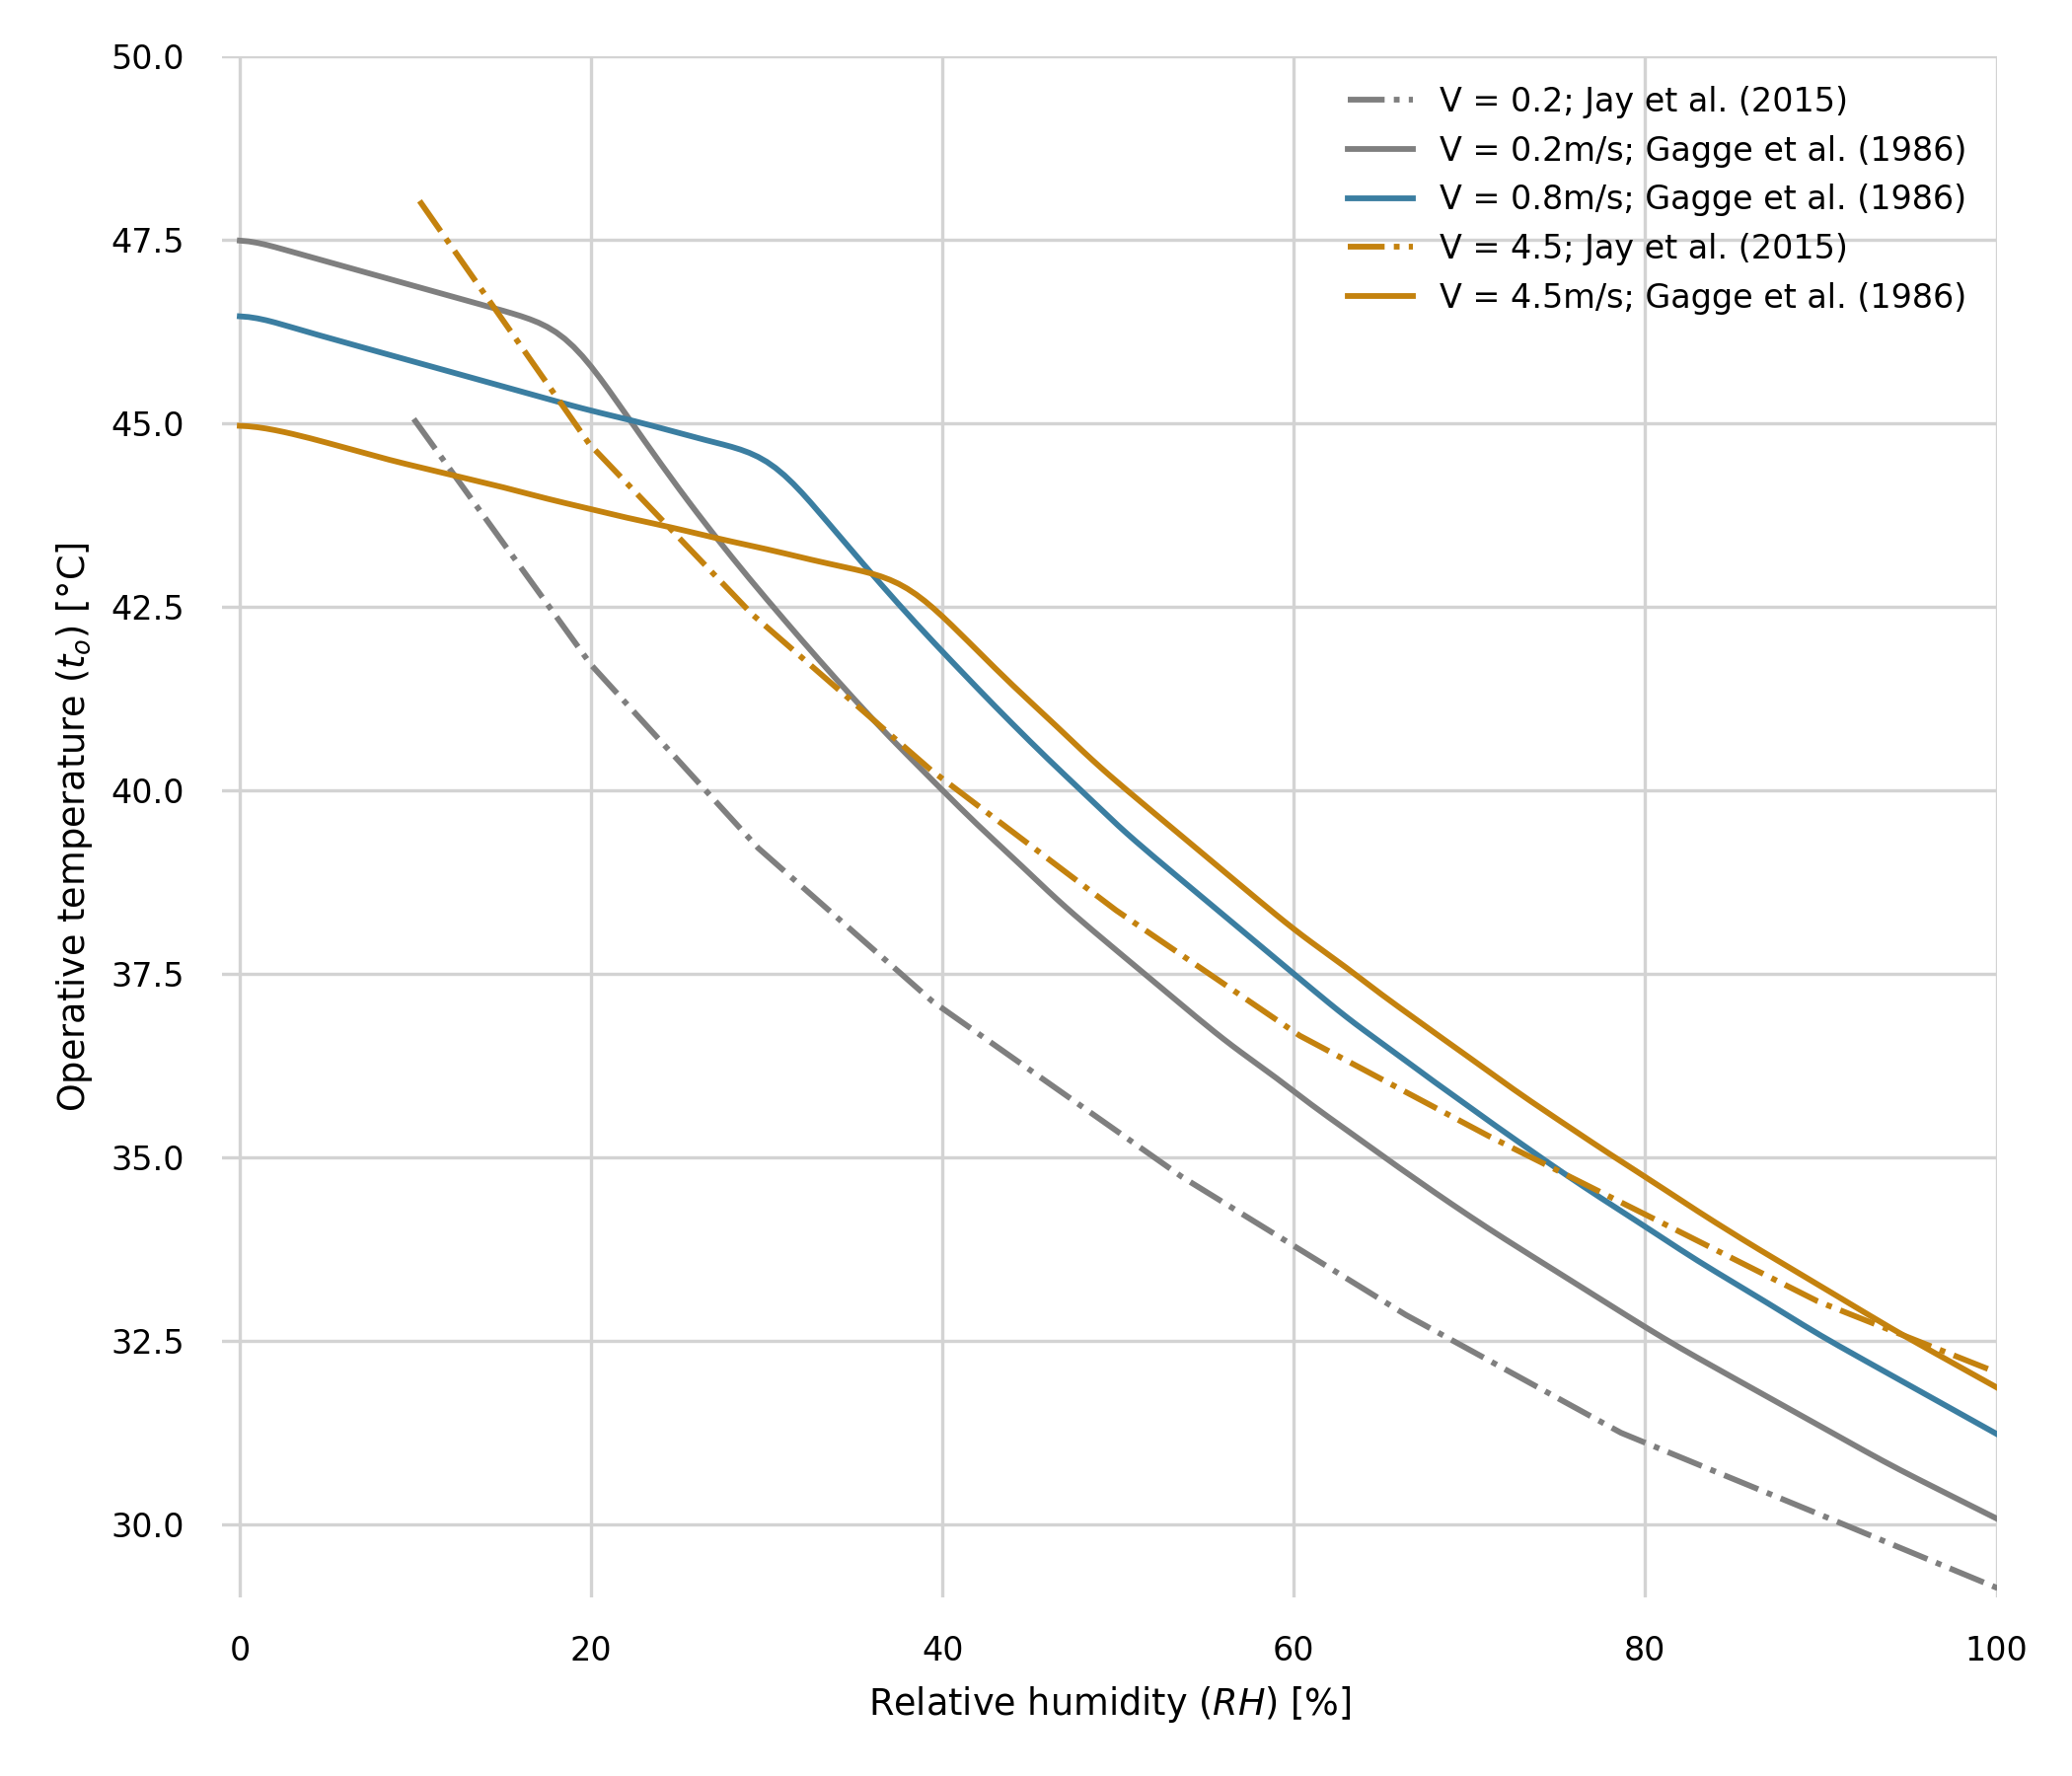
\includegraphics[width=\textwidth]{figures/comparison_air_speed}
    \caption{Predicted limits above which thermal strain is estimated to occur.
    The figure shows the results calculated using the \mycite{GaggeSET} model and the \mycite{Jay2015} models.
    Each line demarcates the point above which heat strain is expected to occur.}
    \label{fig:comparison_air_speed}
\end{figure}

\subsection{Metabolic Rate and Clothing}\label{subsec:met-clo}

To better understand how personal factors would impact the body's ability to dissipate heat, we calculated when heat stress would occur for different combinations of \ac{met} and \ac{clo}.
Results for people wearing light summer clothing (walking shorts, short-sleeve shirt and sandals, \acs{clo}~=~0.36~clo), and office summer clothing (trousers, short-sleeve shirt, and closed shoes \acs{clo}~=~0.5~clo) who are either seated reading or writing (\ac{met}~=~1.0 met) or standing relaxed (\ac{met}~=~1.2~met) are shown in Figure~\ref{fig:met_clo}.
As expected, decreasing both \ac{met} and \ac{clo} has a net positive effect since it reduces both heat gain and thermal resistance, respectively

\begin{figure}[thb!]
    \centering
    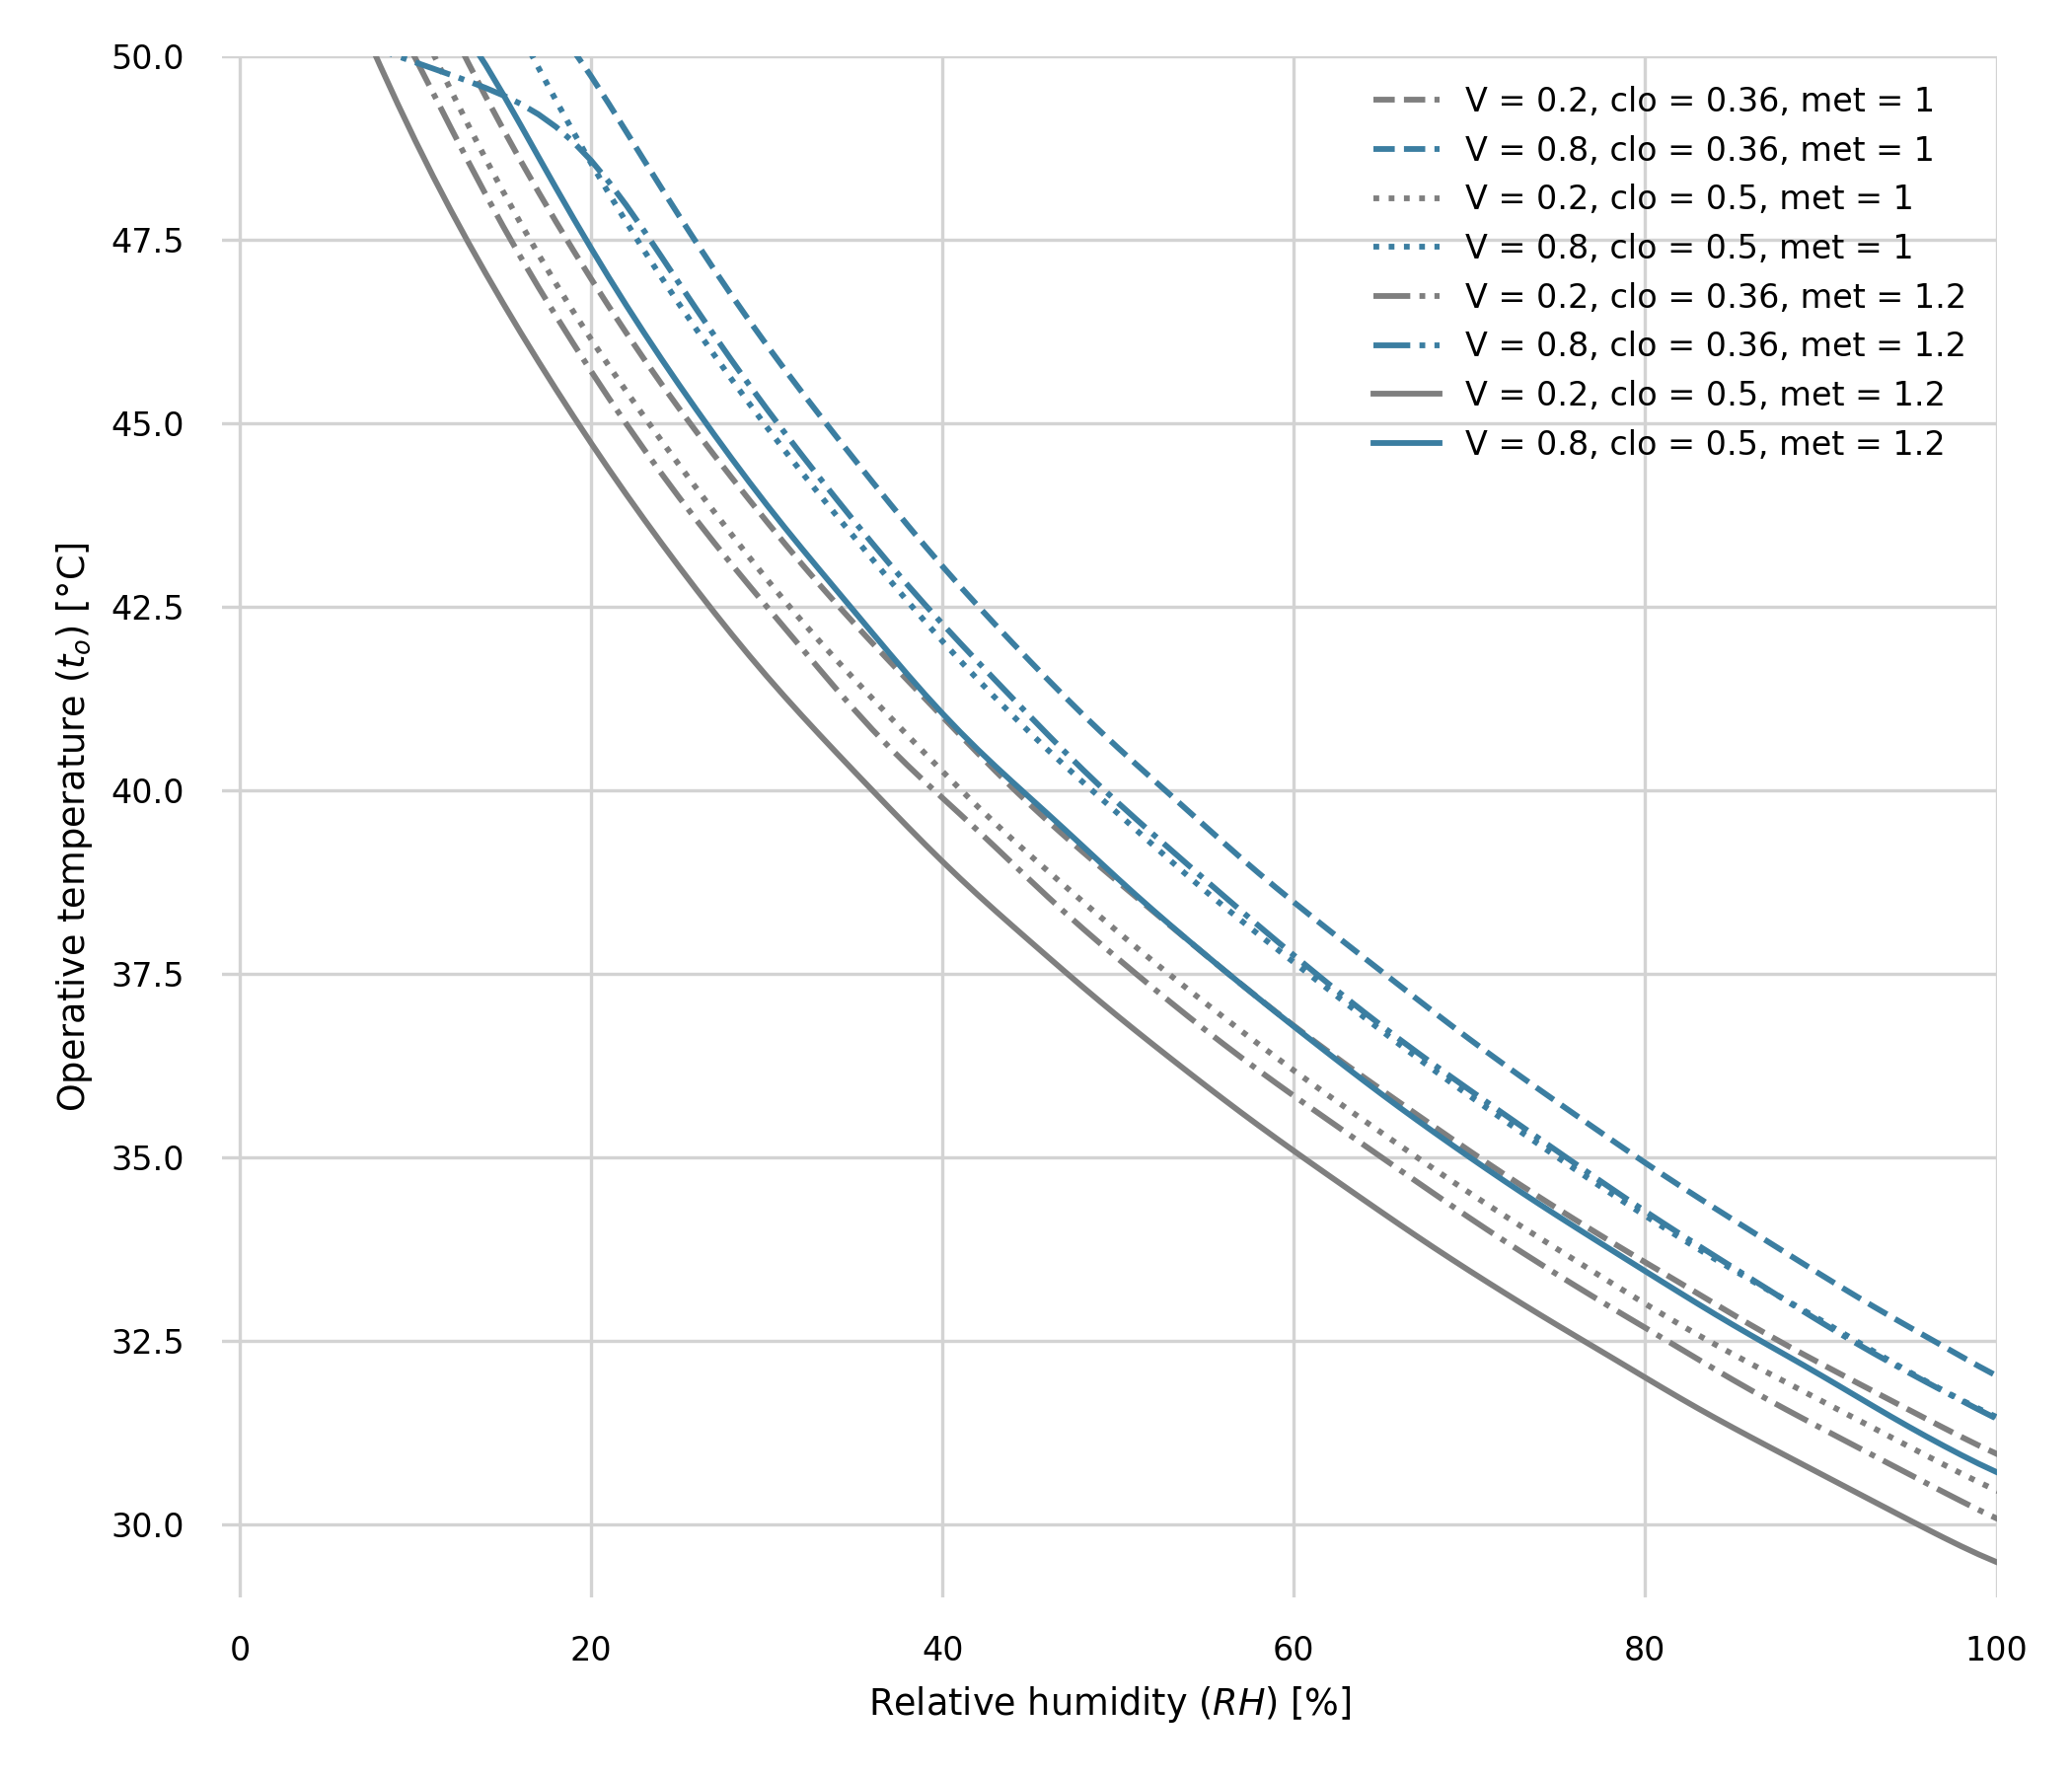
\includegraphics[width=\textwidth]{figures/met_clo}
    \caption{Each line demarcates how different combinations of personal factors (e.g., \ac{met}, \ac{clo}) and environmental factors affect the point above which the body cannot longer dissipate all the endogenous and exogenous heat gains.}
    \label{fig:met_clo}
\end{figure}

\subsection{Model Validation Using Experimental Data}\label{subsec:model-validation-experimental-data}

The environmental conditions above which the use of elevated air speeds would be detrimental according to or model is shown in Figure~\ref{fig:use_fans_experimental}.
We used a red shading to highlight the region in which electric fans should not be used, while we used a green background to depict when elevated air speed can be used to cool the human body.
We also plotted the lines above which thermal stress is expected to occur (see Figure~\ref{fig:comparison_air_speed} for more details).
For a specific value of \ac{rh}, as the value of \ac{v} increases the critical temperature at which thermal stress would occur also increases, as previously stated.
This can be explained that \ac{e-max} increases by a greater amount than and \ac{c-r}.
At the same time, the amount of sweat that the human body can generate is limited and as the value of \ac{t-db} increases, the value of \ac{c-r} also grows.
This causes the body to heats up faster for higher values of \ac{v}.

\begin{figure}[thb!]
    \centering
    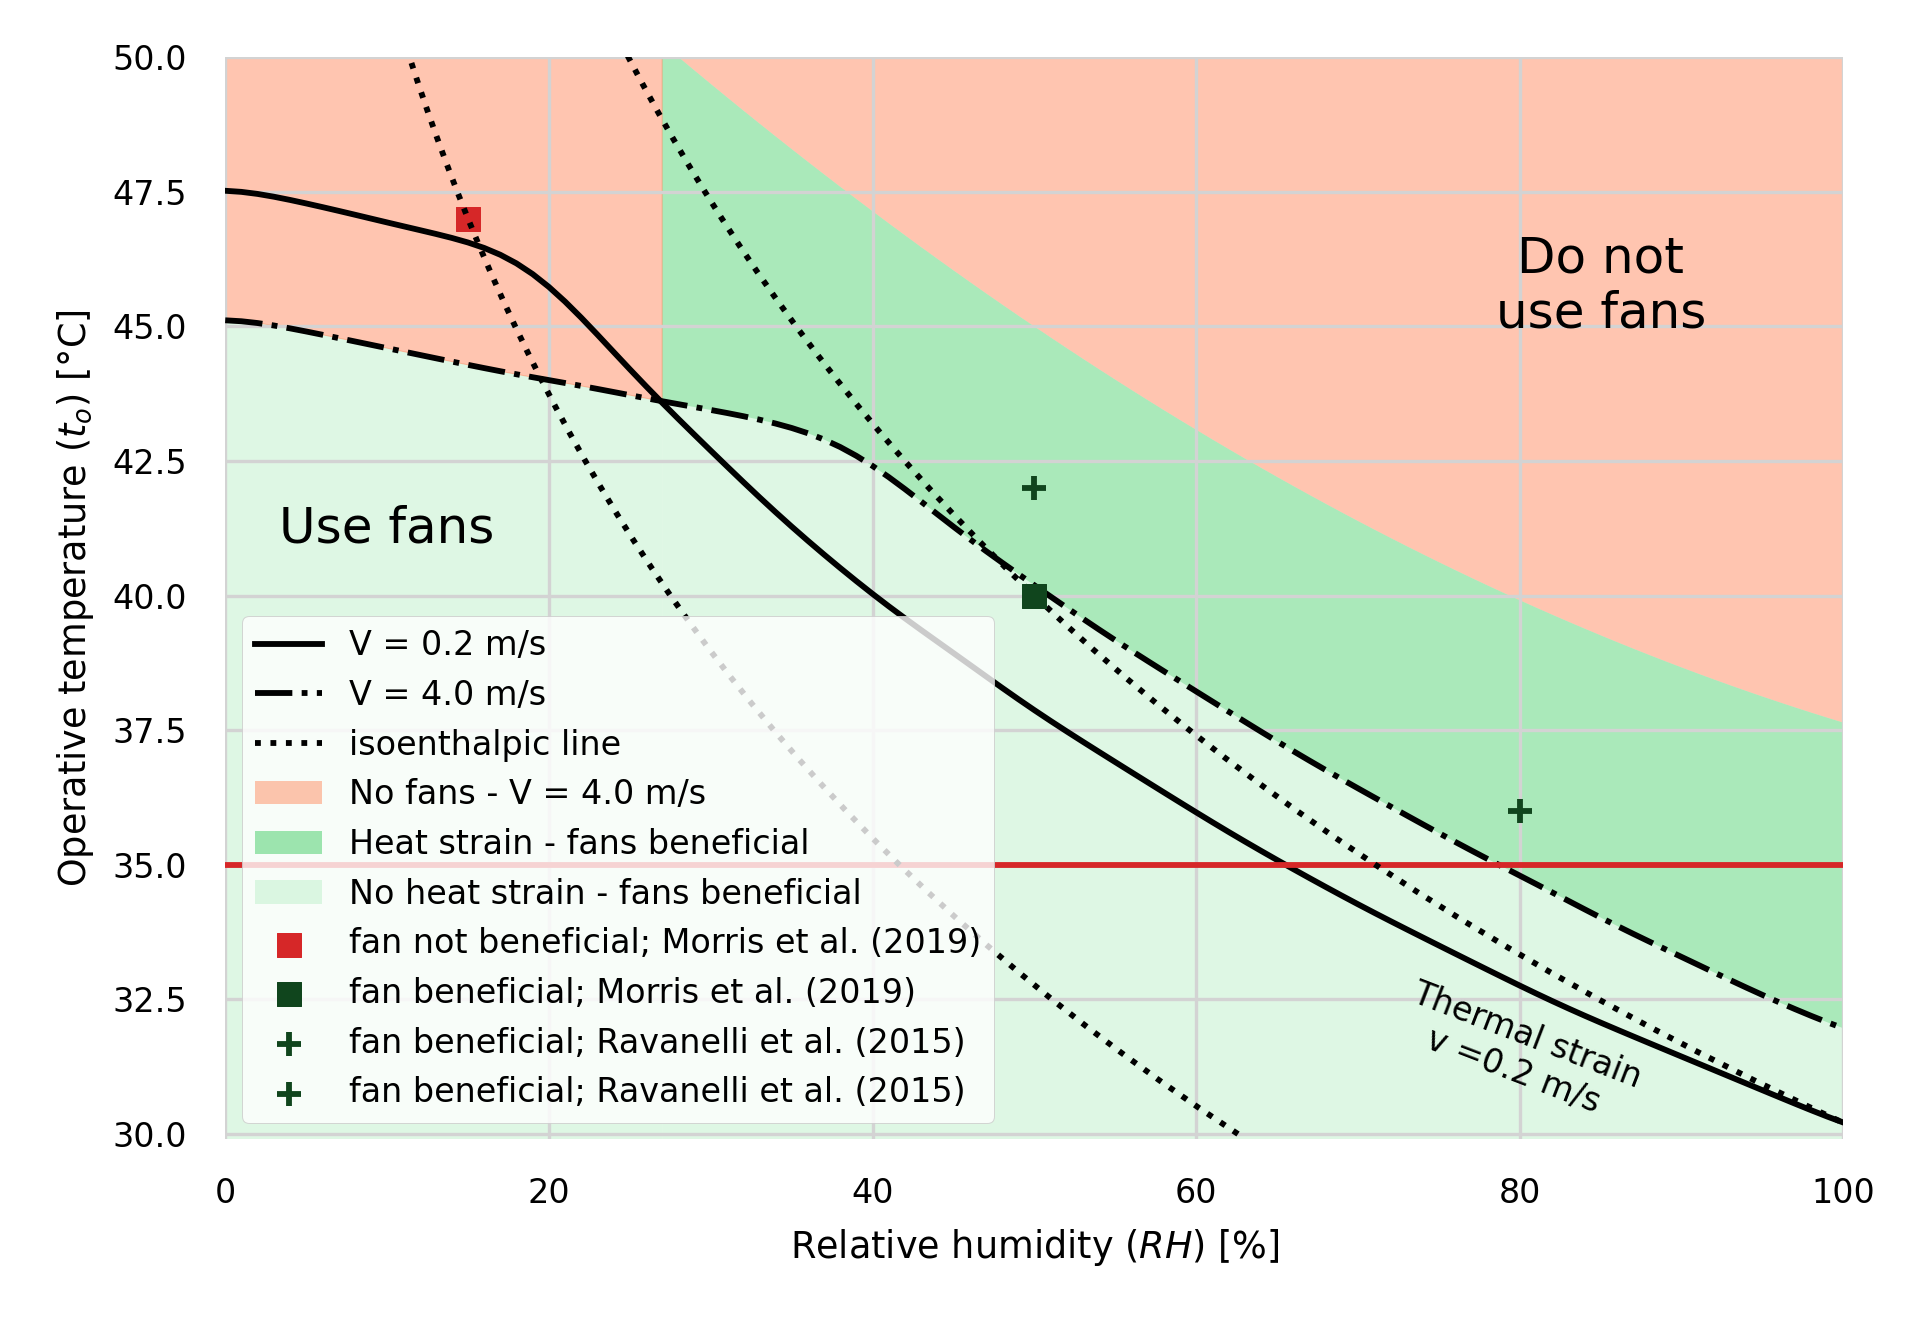
\includegraphics[width=\textwidth]{figures/summary_use_fans_comparison_experimental}
    \caption{The green area shows the environmental conditions in which the use of fans is beneficial since they provide additional cooling to the human body.
    The dark lines demarcate the regions above which thermal stress is predicted to occur for that specific \ac{v}.
    In the hatched area, while the use of fans is still beneficial, people are most likely to suffer from heat strain.
    The red area demarcates the region in which electric fans should not be used.
    }
    \label{fig:use_fans_experimental}
\end{figure}

% note OJ I would expect the curves to bend downwards at very low humidities.
% note OJ I do not think the red dot is necessarily interpreted correctly. This should be "fans detrimental" so should be in the do not use fan area. We have no published the data yet, but this is VERY much the case for the elderly... at 47C/10% fan make things MUCH worse (i.e. genuinely dangerous) - so we do not want to miss this in this model - like we did in our 2015 paper!

% todo compare results in the above figure with the results obtained by Gagnon2017

To validate our results we used experimental data previously published.
In Figure~\ref{fig:use_fans_experimental} we present the results obtained by \mycite{Morris2019} and \mycite{Rate2015}.
The former determined that electric fans (\ac{v}~=~2.0~m/s) are beneficial when \ac{t-db}~=~40~$^{\circ}$C and \ac{rh}~=~51~\%, but should not be used when \ac{t-db}~=~47~$^{\circ}$C and \ac{rh}~=~15~\%.
\mycite{Rate2015} concluded that electric fans (\ac{v}~=~4.0~m/s) help in preventing heat-related elevation in heart rate and \ac{t-cr} in both of the following conditions \ac{t-db}~=~42~$^{\circ}$C and \ac{rh}~=~50~\%, and \ac{t-db}~=~36~$^{\circ}$C and \ac{rh}~=~80~\%.
Our results are in agreement with those obtained by \mycite{Rate2015} and those obtained by \mycite{Morris2019} in which participants were exposed to \ac{t-db}~=~40~$^{\circ}$C and \ac{rh}~=~51~\%.
However, the Gagge model also predicts that the use of electric fans should be beneficial even when \ac{t-db}~=~47~$^{\circ}$C and \ac{rh}~=~15~\%.
This result is in disagreement with the experimental results of \mycite{Morris2019}.
% todo EA This whole validation section is inserted into a section calle 'when can electric fans be used?" This is really hard for the reader. Need to reorganize and separate these issues.

As previously mentioned in the Introduction Section, the enthalpy of the air in \mycite{Morris2019} experiment was lower in the scenario with higher temperature and lower \ac{rh}.
%The black dashed lines, in Figure~\ref{fig:use_fans_experimental}, are isoenthalpic lines passing through the conditions studied by \mycite{Morris2019}.
Evaporative cooling technologies could, therefore, be used to reduce the value of \ac{t-db} and avoid heat strain.
Evaporative cooling can be achieved by spraying water in the air or even by placing wet towels near the electric fan.

\subsection{Benefits of Using Electric Fans}\label{subsec:use-fans}

To understand in which locations worldwide the use of electric fans would be beneficial, in Figure~\ref{fig:energy_storage_delta} we overlaid a plot showing the environmental conditions under which fans can be used with a scatter plot depicting the maximum extreme weather conditions recorded worldwide in more than 5000 stations.
% todo data below are incorrect
We determined that in approximately 97~\% of the locations thermal stress should not occur even without air movement, however, this number increases to 100~\% and 99~\% when \ac{v} is increased to 0.8~m/s and 4.5~m/s, respectively.
The use of fans (\ac{v}~=~0.8~m/s) during heatwaves would be beneficial in all the locations worldwide while in 171 locations heat strain may occur if fans are not used.

\begin{figure}[thb!]
    \centering
    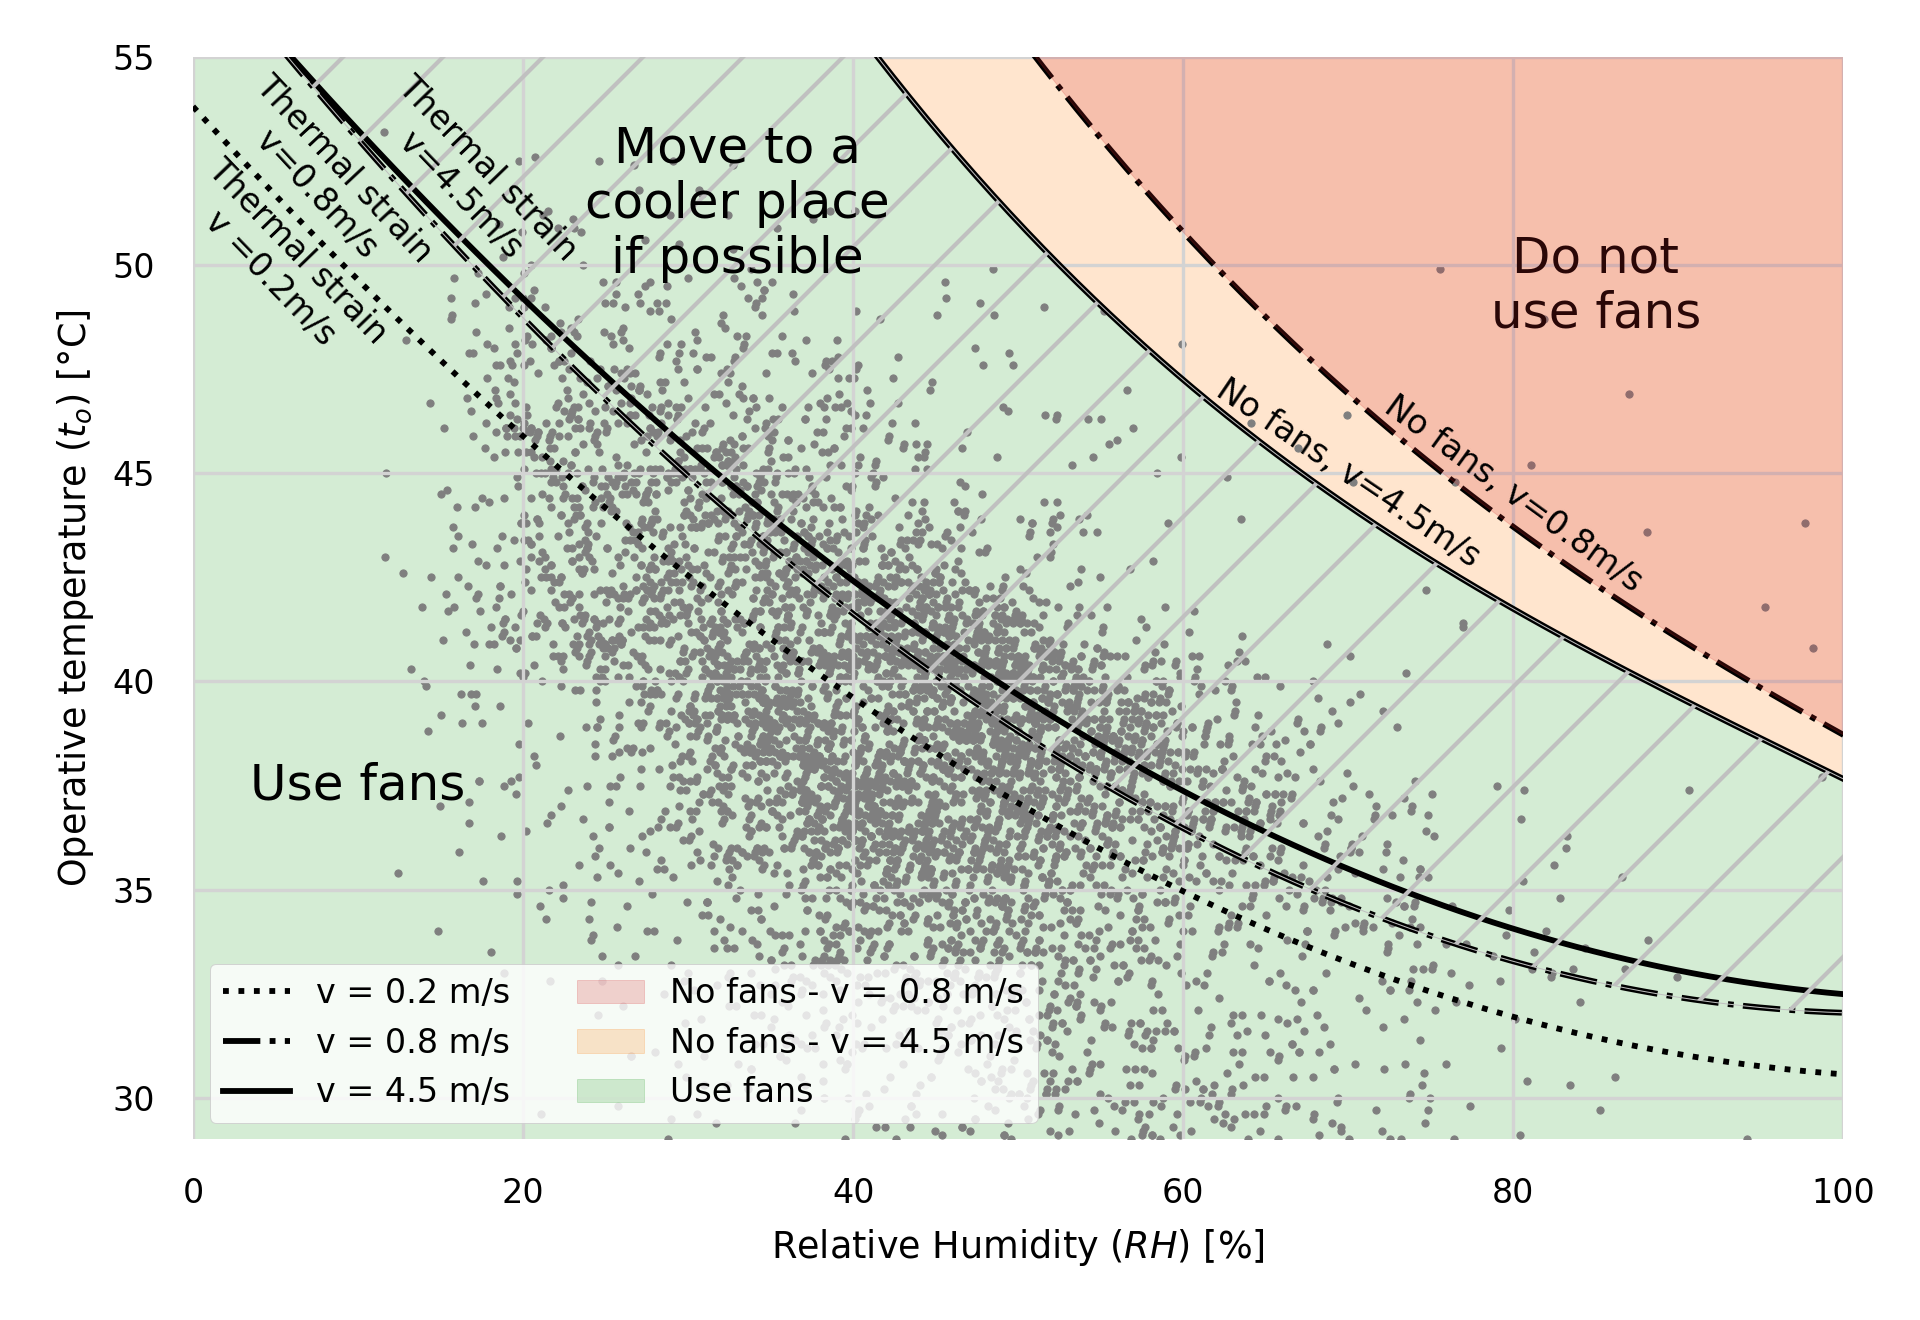
\includegraphics[width=\textwidth]{figures/use_fans}
    \caption{Environmental conditions under which the use of electric fans is beneficial, for more information on how to interpret the Figure please refer to the caption of Figure~\ref{fig:use_fans_experimental}.
    The dots show the maximum extreme climate conditions recorded over the last 20 years in more than 5000 locations worldwide.}
    \label{fig:energy_storage_delta}
\end{figure}

% note OJ I think a lot of the points in the top-left area should be labeled as fans being detrimental

% https://advances.sciencemag.org/content/6/19/eaaw1838

To better quantify how many people would benefit from the use of electric fans we combined the city population with the weather data.
The former contained data from the 115 most populous cities worldwide.
We plotted the data in Figure~\ref{fig:map-population-temperature}.
Each marker shows where the city is located, the dot size is proportional to the number of people living in that urban area, while the color shows the extreme \ac{t-db} recorded in that city.
% todo data below are incorrect
In 2020, a total of approximately 650 million people (8~\% percent of the global population) lived in the urban agglomerate of the 115 largest cities.
In 95 of them, \ac{t-db} higher than 35~$^{\circ}$C\@ were recorded and these cities had a total population of approximately 550 million people.

\begin{figure}[thb!]
    \centering
    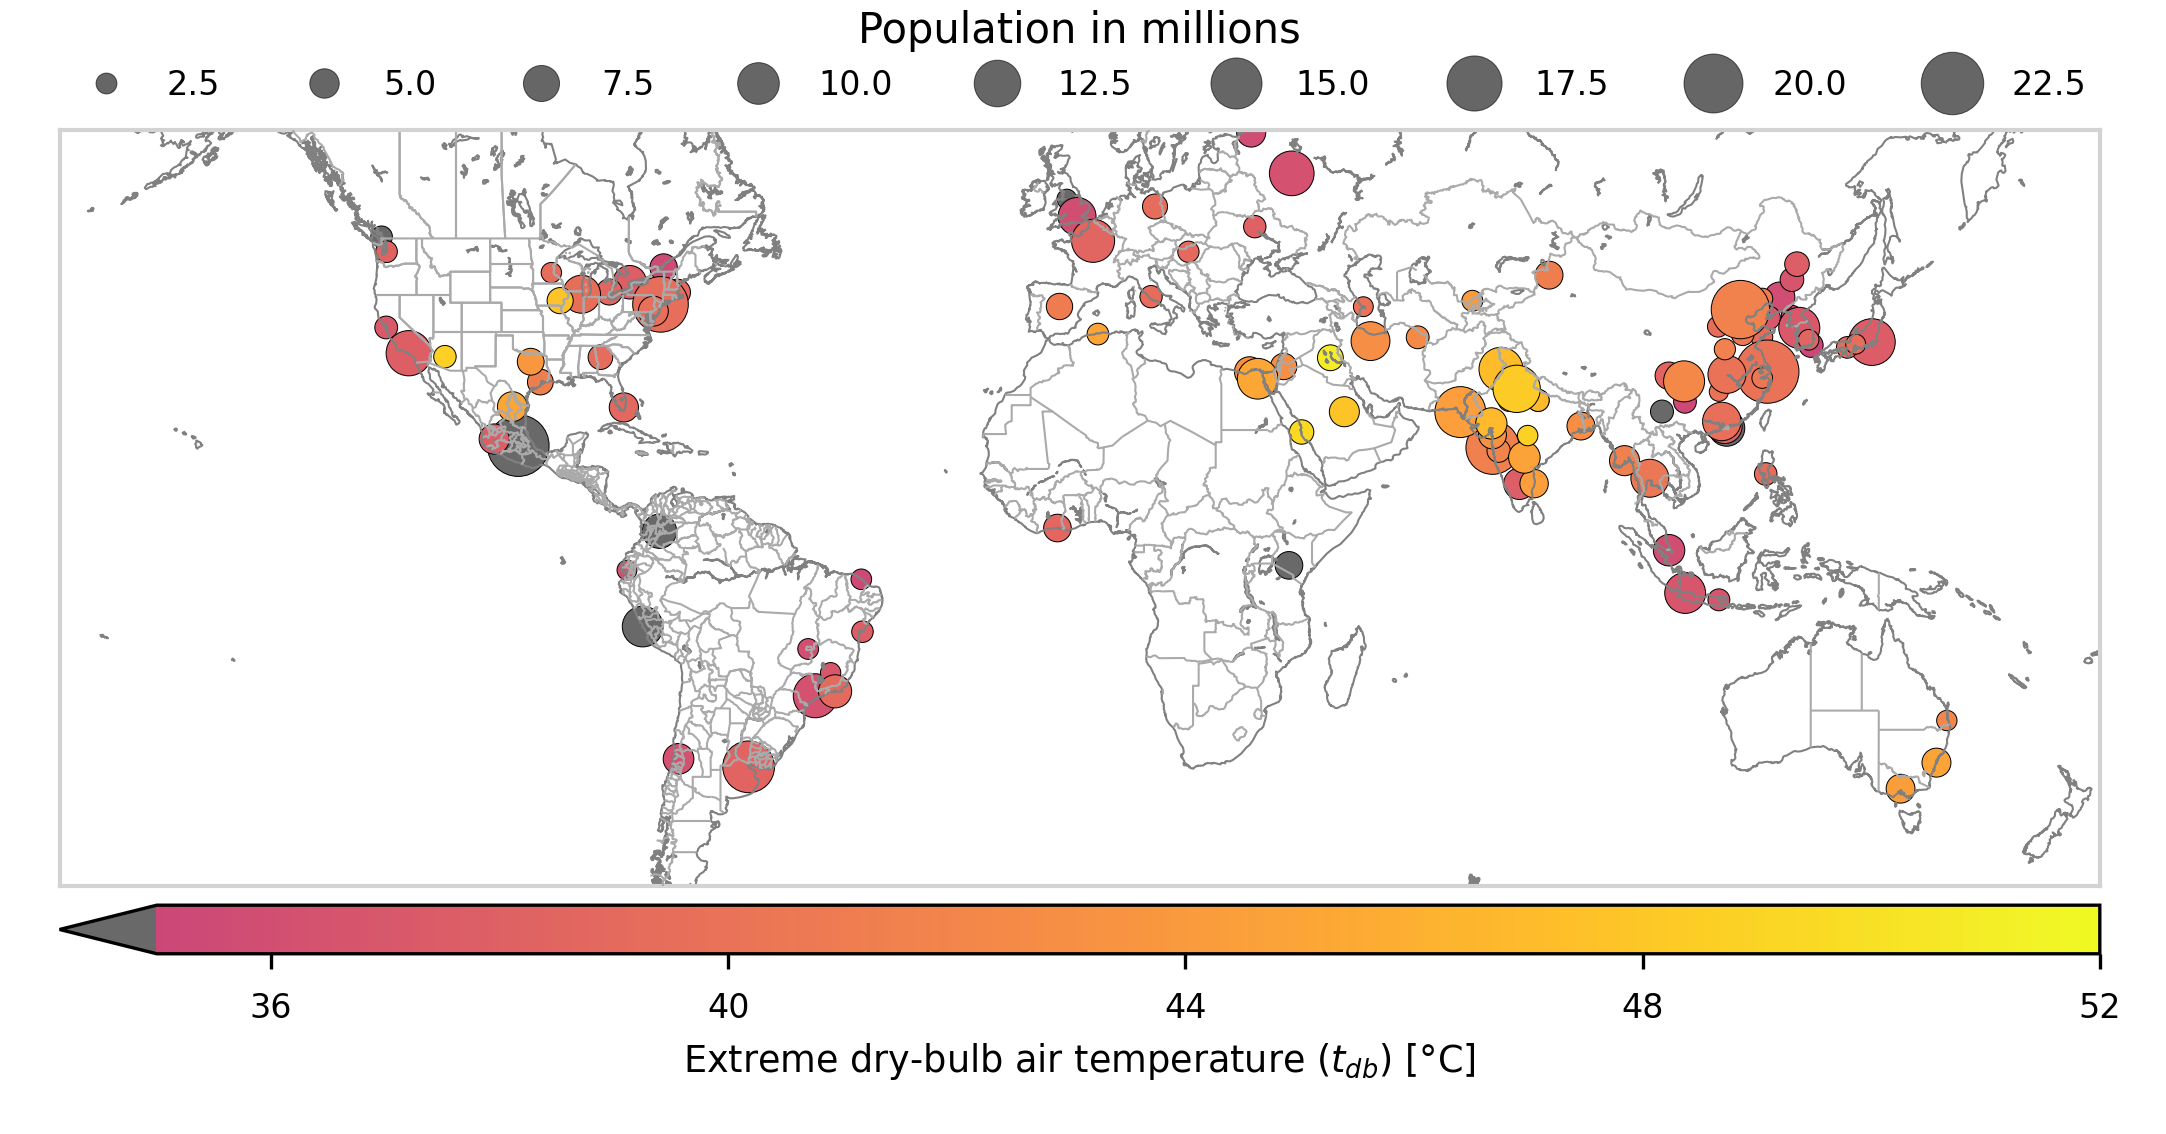
\includegraphics[width=\textwidth]{figures/map-population-temperature}
    \caption{Most populous 115 cities worldwide}
    \label{fig:map-population-temperature}
\end{figure}

% note OJ This is a nice figure but I think we might be overestimating the efficacy of fan use in hot/dry conditions?

We estimated that in all the 115 most populous cities the use of electric fans would be beneficial for healthy adults seated quietly (\ac{met}~=~1.0~met) and wearing a value of \ac{clo} equal to 0.36~clo.
% note OJ It would be great if some kind of economic outcome could be added to this?
The \mycite{GaggeSET} model predicted that healthy adults living in 74 cities (approximately 394 million inhabitants) should not experience heat strain even without increasing air movement.
However, they should still be encouraged in using electric fans to improve their thermal comfort in an energy-efficient way.
An additional 33 million people would avoid heat strain by elevating the air speed up to 0.8~m/s.

\begin{figure}[thb!]
    \centering
    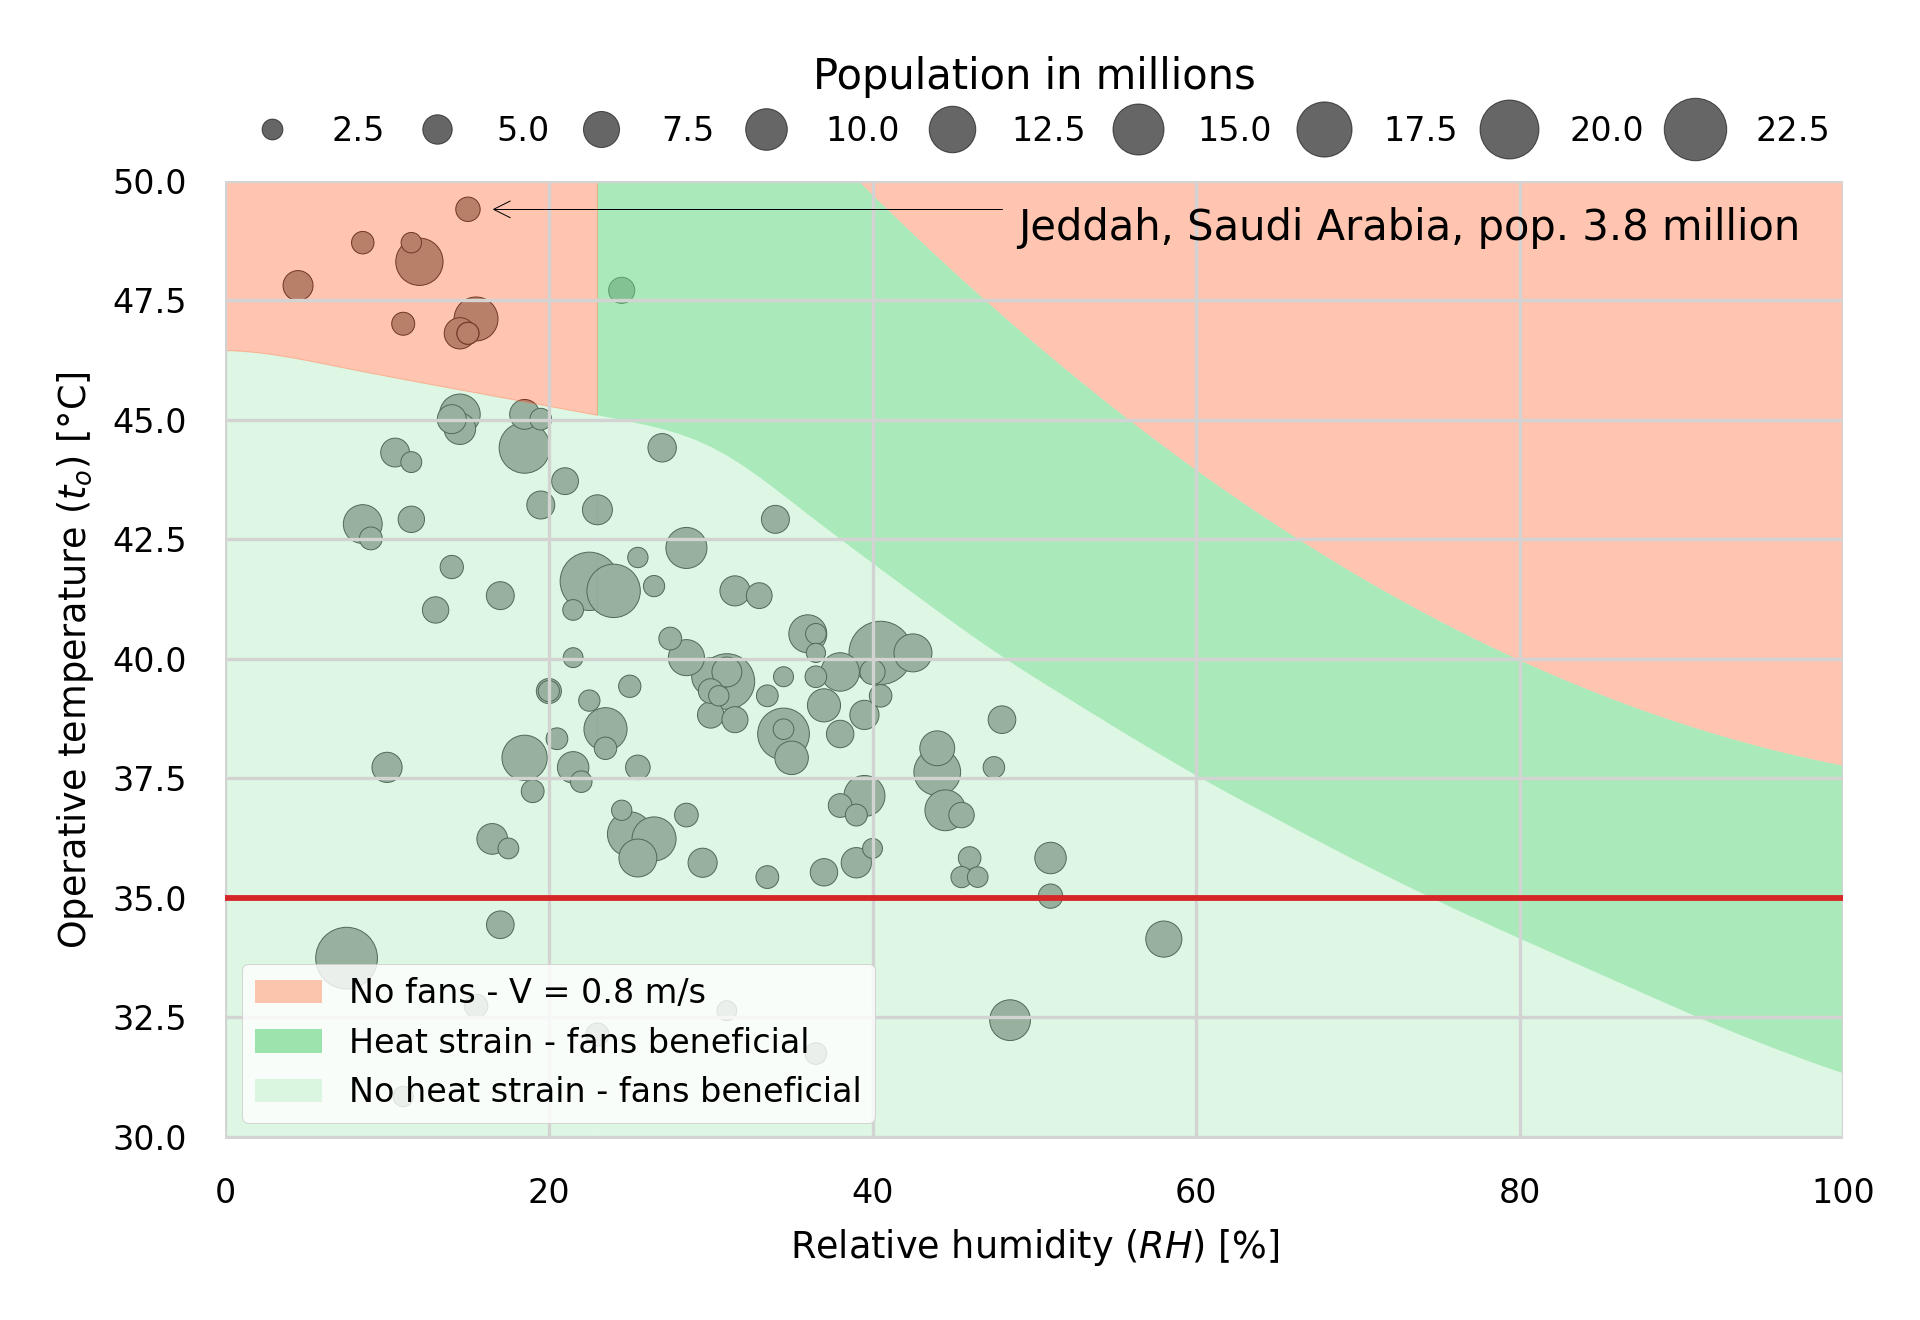
\includegraphics[width=\textwidth]{figures/use_fans_and_population}
    \caption{Environmental conditions under which the use of electric fans is beneficial, for more information on how to interpret the Figure please refer to the caption of Figure~\ref{fig:energy_storage_delta}.
    Each dot shows the maximum extreme climate conditions recorded over the last 20 years in each of the 115 most populous cities worldwide.
    These results were calculated assuming \ac{t-r}~=~\ac{t-db}, \ac{clo}~=~0.35~clo, \ac{met}~=~1.0~met.}
    \label{fig:use_fans_and_population}
\end{figure}

% note OJ Same concern about the top-left area in this figure.

\subsection{Sweat Rate}\label{subsec:sweat-rate}

The predicted values of \ac{m-sweat} at different combinations of \ac{t-db} and \ac{rh} for two values \acf{v}~=~0.2~m/s and 0.8~m/s are shown in Figure~\ref{fig:sweat_rate}.
In most of the combinations of \acf{t-db} and \acf{rh} the predicted values of \ac{m-sweat} are slightly higher in the `still air conditions' than when \ac{v}~=~0.8~m/s for \ac{rh} higher than 20~\%.
On the other hand, \ac{m-sweat} are higher with fan use when \ac{rh} is lower than 10~\%.

% todo better describe this section

\begin{figure}[thb!]
    \centering
    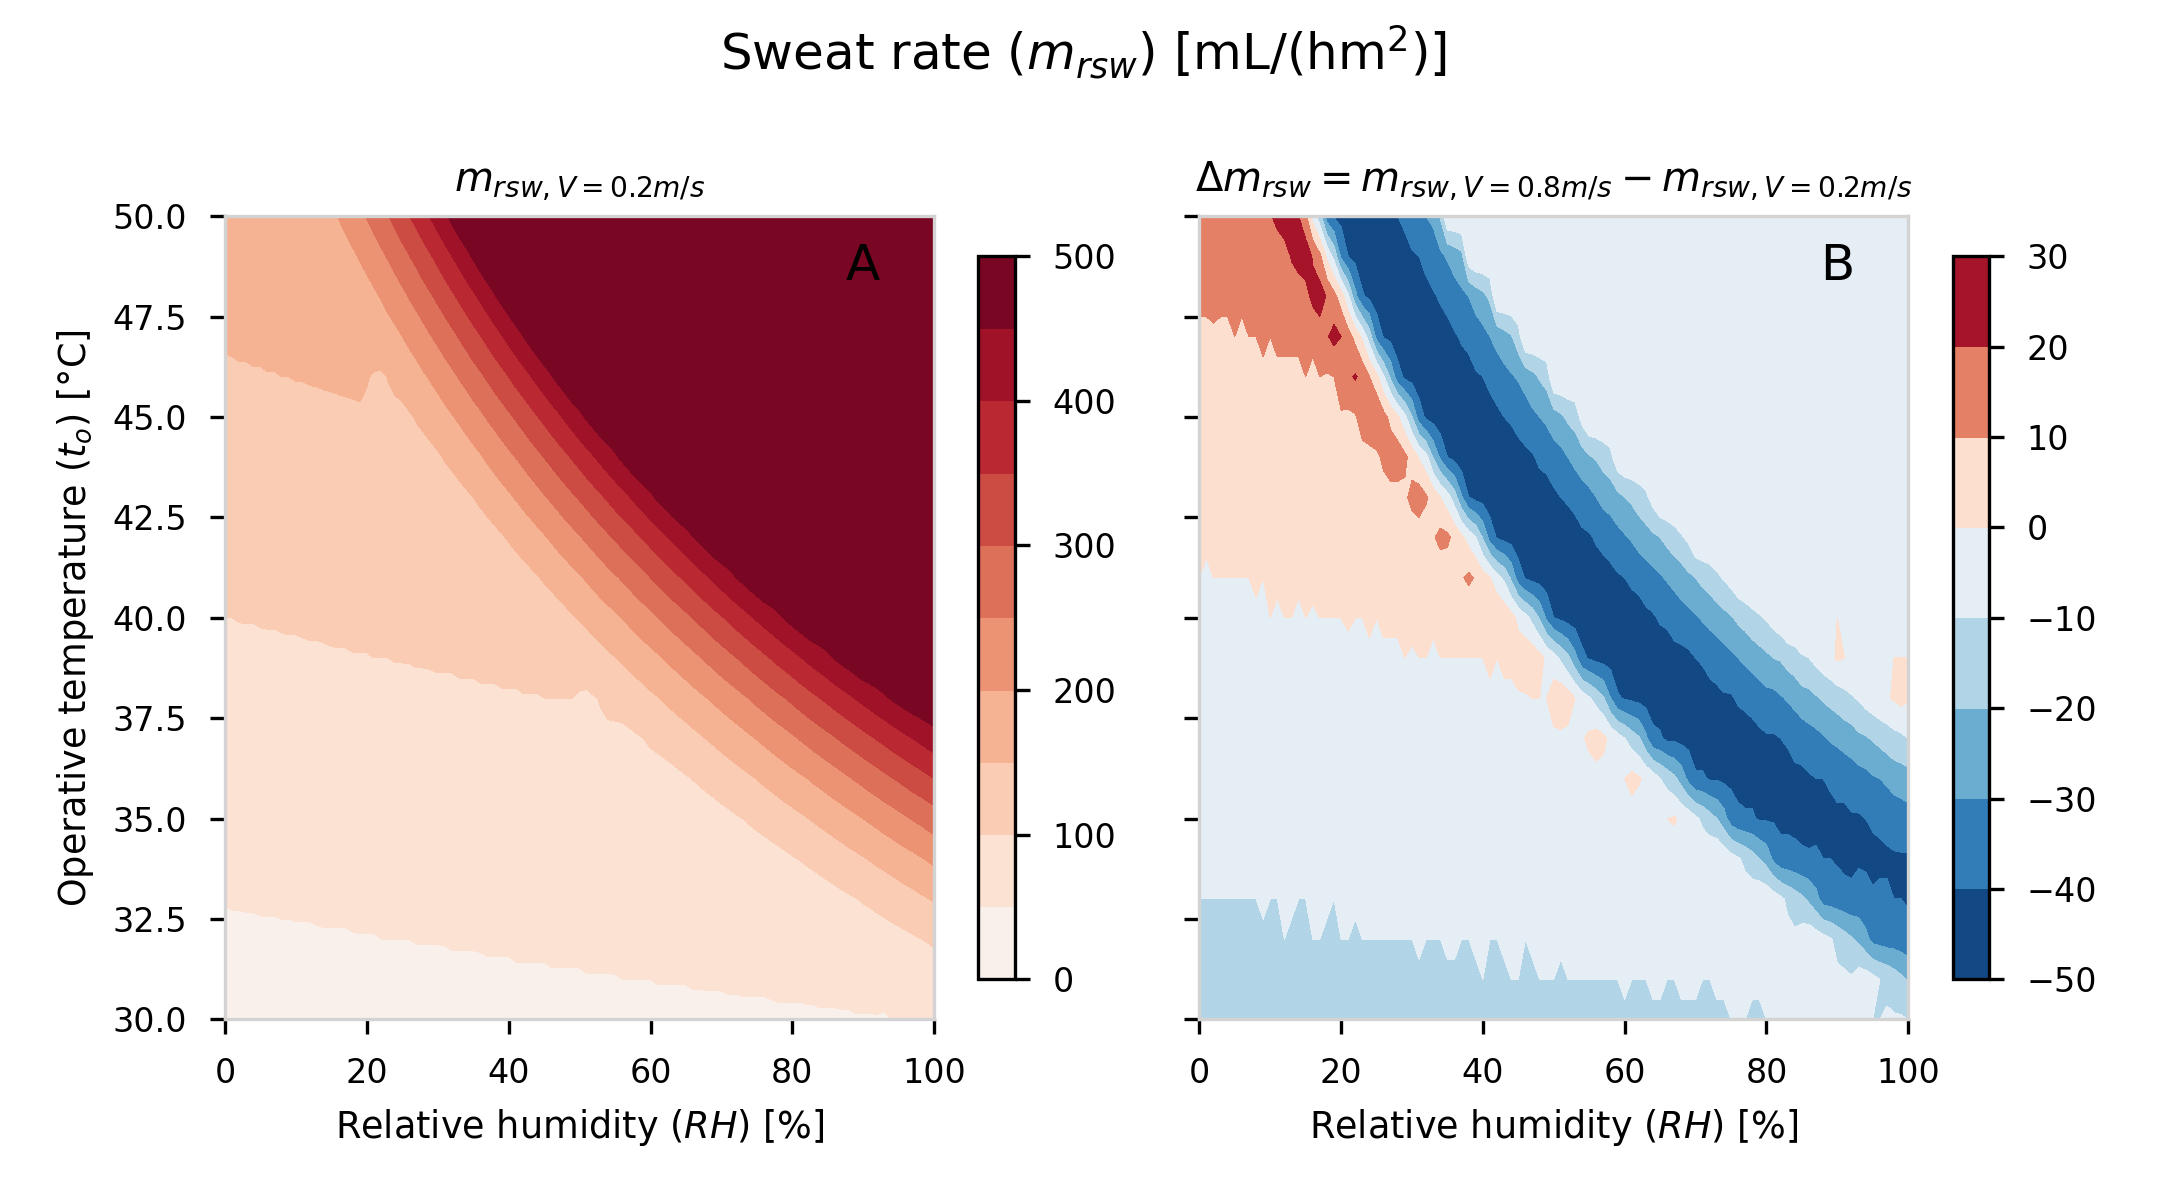
\includegraphics[width=\textwidth]{figures/sweat_rate}
    \caption{Predicted \acf{m-sweat} at different combinations of \acf{t-db} and \acf{rh} for two values \acf{v}~=~0.2~m/s and 0.8~m/s.}
    \label{fig:sweat_rate}
\end{figure}

% note OJ Did you compare these estimated data to those reported in our physiological studies? Might be helpful